% -*- coding=utf-8 -*-
% ============================================================================
% 文件名称：chapter/boyogala5_chapters.tex
% 文件用途：论文正文各章内容汇总（已将原 chapsection 中实际使用的四章内容整合至本文件）
%           1. 第 1 章 绪论（原 chapter/chapsection/00ntroduction.tex）
%           2. 第 2 章 预备知识（原 chapter/chapsection/01Preliminaries.tex）
%           3. 第 3 章 数据预处理（原 chapter/chapsection/02Dataproc.tex）
%           4. 第 4 章 主要内容（原 chapter/chapsection/03myresults.tex）
% ============================================================================

% ============================================================================
% 第 1 章 绪论（转写自 chapter/chapsection/00ntroduction.tex）
% ============================================================================
\chapter{绪论}

\begin{figure}[htp]
	\centering
	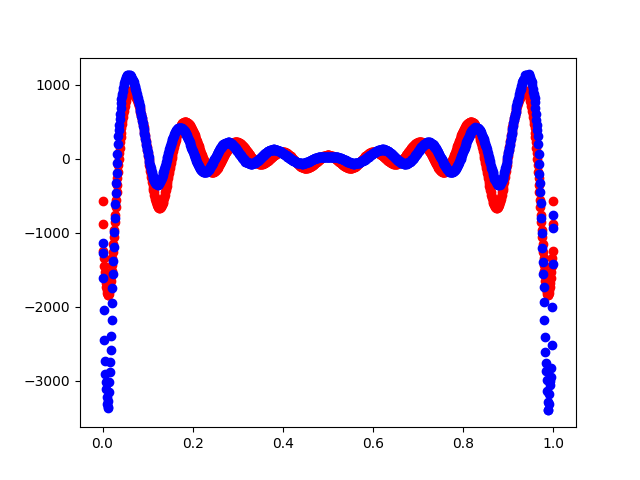
\includegraphics[width=6cm]{figure/model1_1000.png}
	\hspace{1cm}
	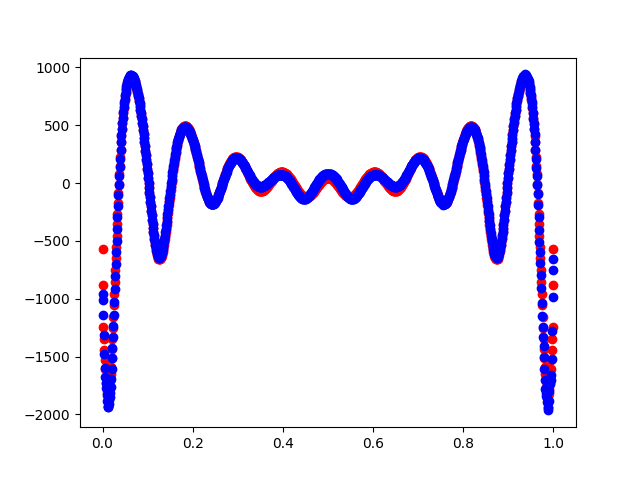
\includegraphics[width=6cm]{figure/model1_10000.png}
	\bicaption{中文题图}
	{English caption}
	\label{fig1}
\end{figure}

\begin{figure}[htp]
    \centering
    
\includegraphics[width=0.5\linewidth]{figure/attention.png}
    \bicaption{中文题图}{English caption}
    \label{fig:placeholder}
\end{figure}

\section{选题来源与背景}

特征值与特征向量问题是线性代数与矩阵理论中的核心内容之一，其数学表述为：对于给定的 $n$ 阶实对称矩阵 $A \in \mathbb{R}^{n \times n}$，寻找标量 $\lambda$ 和非零向量 $x \in \mathbb{R}^n$，使得
\[
Ax = \lambda x
\]
成立，其中 $\lambda$ 称为矩阵 $A$ 的特征值，$x$ 称为对应于 $\lambda$ 的特征向量。若进一步要求 $\|x\|_2 = 1$，则称 $x$ 为单位特征向量。

特征值问题的研究最早可追溯到 18 世纪欧拉（Euler）对刚体转动惯量主轴的研究，以及拉格朗日（Lagrange）和柯西（Cauchy）在力学系统稳定性分析中的工作。19 世纪，随着矩阵理论的建立（凯莱、西尔维斯特等人的贡献），特征值问题被纳入到统一的代数框架之中。20 世纪以来，随着量子力学、振动理论、控制论等学科的发展，特征值问题逐渐成为现代科学与工程计算中不可或缺的工具。

\section{选题目的与意义}

对于实对称矩阵，其特征值均为实数，且可按大小排序为
\[
\lambda_1 \leq \lambda_2 \leq \cdots \leq \lambda_n
\]
其中，最小特征值（第一特征值）$\lambda_1$ 与次最小特征值（第二特征值）$\lambda_2$ 具有特别重要的物理与应用意义：

在主成分分析（PCA）中，协方差矩阵的第一、第二主特征值对应数据方差最大的两个方向，是数据降维与可视化的基础；在谱图理论中，图拉普拉斯矩阵的第二小特征值（代数连通度，Fiedler 值）刻画了图的连通性，与图分割、社区发现密切相关；在结构动力学中，第一、第二阶固有频率（对应于特征值）决定了结构的主要振动模态；在网络分析（如 Google 的 PageRank 算法）中，主特征向量给出了网页的重要性排序。由瑞利商（Rayleigh quotient）理论可知，第一特征值满足极值刻画：
\[
\lambda_1 = \max_{x \neq 0} \frac{x^{\mathrm{T}} A x}{x^{\mathrm{T}} x}
\]
而第二特征值则由 Courant--Fischer 极小极大定理给出：
\[
\lambda_2 = \max_{\substack{x \neq 0 \\ x \perp v_1}} \frac{x^{\mathrm{T}} A x}{x^{\mathrm{T}} x}
\]
其中 $v_1$ 为第一特征值对应的特征向量。这一变分刻画为采用优化算法求解特征值提供了理论桥梁。

本研究将数值代数中的特征值问题与群体智能优化方法相结合，深化了对瑞利商变分原理的理解与应用，丰富了特征值求解的方法体系，为以优化视角处理代数问题提供了实例与思路。

应用意义：

基于 PSO 的方法不依赖矩阵的可微性与特殊结构，对于一些传统方法难以处理的非常规问题（如带复杂约束的广义特征值问题）具有潜在的适用性；算法的并行性良好，适合在现代多核与分布式计算环境下实现，便于扩展到大规模问题；第一、第二特征值在 PCA、谱聚类、图分割、振动分析等众多领域有直接应用，本研究的成果可为这些应用领域提供新的计算工具。

\section{国内外文献综述}

传统的特征值求解方法主要包括幂法（Power Method）、反幂法、QR 算法、Jacobi 方法、Lanczos 方法等。这些方法在精度和稳定性方面表现优异，但也存在一定局限：

幂法对特征值分布敏感，当 $|\lambda_1|$ 与 $|\lambda_2|$ 接近时收敛缓慢；QR 算法计算复杂度较高（$O(n^3)$），且对初值和矩阵结构有一定要求；部分方法在处理大规模稀疏矩阵或病态矩阵时面临数值不稳定问题。正是由于上述瑞利商所揭示的特征值问题与优化问题的等价性，使得将群体智能优化算法应用于特征值求解成为可能。粒子群优化算法（Particle Swarm Optimization, PSO）作为一种典型的群体智能方法，具有原理简单、参数少、全局搜索能力强、不依赖目标函数梯度信息等优点，为特征值问题提供了一条新的求解途径。

特征值问题的经典数值方法已发展得较为成熟。Golub 与 Van Loan 在其经典著作《Matrix Computations》中系统总结了 QR 算法、幂法、Lanczos 方法等的理论与实现。幂法及其变体（反幂法、移位幂法）由于实现简单，常用于求解主特征值；但当 $\lambda_1$ 与 $\lambda_2$ 的比值 $|\lambda_2 / \lambda_1|$ 接近 1 时，其收敛速度显著下降。

QR 算法是求解中小规模稠密矩阵全部特征值的标准方法，由 Francis 与 Kublanovskaya 于 20 世纪 60 年代提出，具有良好的数值稳定性。对于大规模稀疏对称矩阵，Lanczos 方法及其重正交化变体得到了广泛应用。此外，Davidson 方法、Jacobi-Davidson 方法在量子化学计算中求解极端特征值方面表现出色。

尽管这些方法体系完整、精度高，但它们大多基于矩阵分解或迭代收缩，在面对非标准的约束条件或非线性扩展时，往往需要重新设计算法。

粒子群优化算法由 Kennedy 与 Eberhart 于 1995 年首次提出，其灵感来源于鸟群觅食的群体行为。在标准 PSO 中，每个粒子 $i$ 的位置 $x_i$ 与速度 $v_i$ 按如下规则更新：
\begin{equation}
 v_i^{t+1} = w \cdot v_i^t + c_1 r_1 (p_i - x_i^t) + c_2 r_2 (g - x_i^t)   
\end{equation}
\[
x_i^{t+1} = x_i^t + v_i^{t+1}
\]
其中 $w$ 为惯性权重，$c_1, c_2$ 为学习因子，$r_1, r_2$ 为 $[0,1]$ 上的随机数，$p_i$ 为粒子的个体历史最优位置，$g$ 为群体全局最优位置。

为提升算法性能，学者们提出了诸多改进：Shi 与 Eberhart 引入惯性权重以平衡全局与局部搜索能力；Clerc 与 Kennedy 提出收缩因子（constriction factor）模型以保证算法收敛性；此后又出现了自适应 PSO、量子行为 PSO（QPSO）、混合 PSO 等多种变体。这些研究表明，PSO 在连续优化问题中具有良好的全局搜索能力，但也存在易陷入局部最优、后期收敛速度慢等问题。

将智能优化算法用于特征值求解的研究近年来逐渐增多。早期有学者利用神经网络（如 Hopfield 网络、递归神经网络）求解实对称矩阵的特征值与特征向量，将瑞利商作为能量函数构造动力系统。

在群体智能方面，已有研究将遗传算法（GA）、差分进化（DE）等用于求解最大/最小特征值。针对 PSO，部分文献探索了利用 PSO 求解主特征值的方法，其核心思想是将瑞利商作为适应度函数，在单位球面约束下搜索最优向量。这类研究验证了 PSO 求解特征值的可行性，但多数仅关注单个极端特征值，对于第二乃至更多特征值的连续求解、单位特征向量的约束处理以及正交约束的实现，仍有进一步研究的空间。

\section{研究内容}

本文的主要研究目的包括：

建立特征值问题的优化模型：基于瑞利商的极值特性以及 Courant--Fischer 定理，将第一、第二特征值及其单位特征向量的求解转化为带约束的优化问题；

设计基于 PSO 的求解算法：针对单位特征向量的约束条件 $\|x\|_2 = 1$ 与正交约束 $x \perp v_1$，设计相应的适应度函数与约束处理策略，构造可行的粒子群求解框架；

实现连续求解机制：在求得第一特征值与特征向量的基础上，通过收缩（deflation）或正交投影技术，连续求解第二特征值及其单位特征向量；

进行数值实验验证：通过与传统方法（如幂法、QR 算法）的对比，验证所提算法的有效性、精度与适用范围。

\begin{table}[!ht]
	\bicaption{中文图名}{english name}\label{tab:lable}
	\begin{tabular*}{\hsize}{@{}@{\extracolsep{\fill}}lllllllllllll@{}}
		\toprule
		$p_{t}$  &21  &22  &20  &15  &10  &8   &5   &10  &18  &10  &14  &18\\
		\midrule
		$c_{t}$  &5   &13  &10  &10  &10  &10  &10  &10  &10  &10  &10  &10\\
		$h_{t}$  &10  &5   &5   &5   &5   &5   &5   &5   &5   &5   &5   &5 \\
		$s_{t}$  &100 &100 &100 &100 &100 &100 &100 &100 &100 &100 &100 &100\\
		$d_{t}$  &30  &45  &50  &55  &45  &55  &90  &80  &90  &65  &80  &70 \\
		\bottomrule
	\end{tabular*}
\end{table}

\section{本章总结}

第一章，介绍选题背景、目的与意义、国内外文献综述以及本文的主要研究内容。
第二章，介绍平均相对误差的定义、数据拟合方法及数据预处理过程。
第三章，介绍分段拟合方法的实现过程、精度评估及剩余放电时间计算。
第四章，介绍通用模型的构建方法、精度评估及 55A 放电曲线的预测。
第五章，分析衰减特性并建立预测模型，预测不同衰减状态下剩余放电时间。

% ============================================================================
% 第 2 章 预备知识（转写自 chapter/chapsection/01Preliminaries.tex）
% ============================================================================
\chapter{预备知识}
我是预备知识

在离散数学中，图（Graph）是用于表示物体与物体之间存在某种关系的结构。数学抽象后的“物体”称作节点或顶点（英语：Vertex，node或point），节点间的相关关系则称作边。\upcite{bierlich2022comprehensive}在描绘一张图的时候，通常用一组点或小圆圈表示节点，其间的边则使用直线或曲线。

用$\mathbb{R}$和$\mathbb{R}^{n}$分别表示实数域和$n$维实数域. 对任意的实数$x \in \mathbb{R}$, $\lfloor x \rfloor$是向下取整函数，表示不大于$x$的最大整数，且$ \lfloor x \rfloor \leq x$；$\lceil x \rceil$是向上取整函数，表示不小于$x$的最小整数，且$\lceil x \rceil \geq x$.
 
\section{向量、矩阵和范数}
二维平面上的一点$P=(x,y)^{\top}$

\begin{lemma}\label{Lemma4EmYqK}
	假设$e_p,~p=1,2,\cdots,m$是$m$维单位矩阵的第$p$列和列向量$Y_{q} = \left( y_{1,q}, y_{2,q}, \cdots, y_{m,q} \right)^\top \in \mathbb{R}^{m}$, 且$y_{p,q} \neq 0$,  则
	\begin{equation*}
	 \left( e_1, \cdots,e_{p-1}, Y_{q}, e_{p+1}, \cdots, e_m \right)^{-1}  = 
	  	   		\begin{pmatrix} 
		  		1 	   & 0      & \cdots  & 0 			  & -\frac{y_{1,q}}{y_{p,q}}  	& 0 	& \cdots   & 0\\
		  		0 	   & 1      & \cdots  & 0 			  & -\frac{y_{2,q}}{y_{p,q}}  	& 0 	& \cdots   & 0\\
		  		\vdots & \vdots & \ddots  & \vdots 	      &  \vdots     	& \vdots  	& \ddots  & \vdots\\
		  		0      & 0      & \cdots  & 1  			  & -\frac{y_{p-1,q}}{y_{p,q}}  	& 0 	& \cdots   & 0\\	  		
		  		0      & 0      & \cdots  & 0  			  & \frac{1}{y_{p,q}}  	& 0 	& \cdots   & 0\\
		  		0      & 0      & \cdots  & 0  			  & -\frac{y_{p+1,q}}{y_{p,q}}  	& 1 	& \cdots   & 0\\
		  		\vdots & \vdots & \ddots  & \vdots  	  & \vdots  		& \vdots  	& \ddots   & \vdots\\	
		  		0      & 0      & \cdots  & 0  			   & -\frac{y_{m,q}}{y_{p,q}}     & 0     & \cdots   & 1\\	  		
			\end{pmatrix} .
	\end{equation*}
\end{lemma}

\section{开集和闭集}
以$x \in \mathbb{R}^{n}$为球心，$r > 0$为半径的开球记为 
\begin{equation*}
    \mathcal{B}\left(x,r\right) \triangleq \left\{ y \in \mathbb{R}^{n} : \Vert y - x \Vert_{2} < r \right\}
\end{equation*}
和相应的闭球
\begin{equation*}
    \overline{\mathcal{B}}\left(x,r\right) \triangleq \left\{ y \in \mathbb{R}^{n} : \Vert y - x \Vert_{2} \leq r \right\}.
\end{equation*}

\begin{definition}\label{Chapter0Open}
    设非空集合$\mathcal{S} \subseteq \mathbb{R}^{n}$. 若对任意的$x \in \mathcal{S}$, 总存在$r > 0$, 使得$\mathcal{B}\left(x,r\right) \subseteq \mathcal{S}$, 则称$\mathcal{S}$为\textbf{开集}. \textbf{补集}$~\mathcal{S}^{\mathrm{c}} \triangleq \left\{ x \in \mathbb{R}^{n} : x \notin \mathcal{S} \right\}$为开集的集合$\mathcal{S}$称为\textbf{闭集}，其中\textbf{补集}$~\mathcal{S}^{\mathrm{c}}$也被记为$~\overline{\mathcal{S}}$.
\end{definition}

显然地，开球$\mathcal{B}\left(x,r\right)$和闭球$\overline{\mathcal{B}}\left(x,r\right)$分别是开集和闭集. 包含点$x \in \mathbb{R}^{n}$的开集称为$x$的一个\textbf{邻域}. 全空间$\mathbb{R}^{n}$和空集$\emptyset$既是开集又是闭集. 进一步地，
\begin{itemize}
 \setlength{\itemsep}{0pt}
 \setlength{\parsep}{0pt}
 \setlength{\parskip}{0pt}
     \item[$(1)$] 有限个开集$S_i(i=1,\cdots,m)$的交集$\bigcap_{i=1}^{m}S_i$是开集，任意个开集$S_i(i \in \mathcal{I} )$的并集$\bigcup_{i \in \mathcal{I}}S_i$是开集，其中$\mathcal{I}$为有限或无限的指标集合；
     \item[$(2)$] 有限个闭集$S_i(i=1,\cdots,m)$的并集$\bigcup_{i=1}^{m}S_i$是闭集，任意个闭集$S_i(i \in \mathcal{I} )$的交集$\bigcap_{i \in \mathcal{I}}S_i$是闭集，其中$\mathcal{I}$为有限或无限的指标集合.
\end{itemize}

给定一个非空集合$\mathcal{S} \subseteq \mathbb{R}^{n}$与点$x \in \mathcal{S}$, 若存在$r > 0$, 使得$\mathcal{B}\left(x,r\right) \subseteq \mathcal{S}$, 则称$x$为$\mathcal{S}$的\textbf{内点}. 非空集合$\mathcal{S}$中所有\textbf{内点}构成的集合称为$\mathcal{S}$的\textbf{内部},记为$\mathrm{int}\,\mathcal{S}$. 显然，$\mathrm{int}\,\mathcal{S}$是开集，这是因为在$\mathrm{int}\,\mathcal{S}$中的任何一个点，都可找到一个属于$\mathrm{int}\,\mathcal{S}$的开球. 另外，称包含$\mathcal{S}$的最小闭集，即所有包含$\mathcal{S}$的闭集的交集，为$\mathcal{S}$的\textbf{闭包}, 记为$\mathrm{cl}\,\mathcal{S}$. 属于$\mathrm{cl}\,\mathcal{S}$但不属于$\mathrm{int}\,\mathcal{S}$的所有点构成的集合称为$\mathrm{int}\,\mathcal{S}$的边界，记为$\mathrm{bd}\,\mathcal{S}$. 如果存在一个充分大的数$r > 0$, 使得$\mathcal{S} \subseteq \mathcal{B}\left(0,r\right)$, 则称$\mathcal{S}$是\textbf{有界}. 进一步地，称\textbf{有界闭集}$\mathcal{S}$为\textbf{紧集}. 注意，此处的\textbf{紧集}的定义只适合有限维空间.

\section{凸集和凸函数}
图中的边可以是有方向或没有方向的。例如在一张图中，如果节点表示聚会上的人，而边表示两人曾经握手，则该图就是没有方向的，因为甲和乙握过手也意味着乙一定和甲握过手。相反，如果一条从甲到乙的边表示甲欠乙的钱，则该图就是有方向的，因为“曾经欠钱”这个关系不一定是双向的。前一种图称为无向图，后一种称为有向图。

\begin{definition}\label{Chapter0Cone}
    设非空集合$\mathcal{C} \subseteq \mathbb{R}^{n}$. 如果满足对任意的$x \in \mathcal{C}$和$\alpha \in [0,+\infty)$, 都有$\alpha x \in \mathcal{C}$, 则称$\mathcal{C}$为\textbf{锥}.
\end{definition}

从锥的定义 \ref{Chapter0Cone} 可知，锥$\mathcal{C}$是包含所有以原点为起点，并通过$\mathcal{C}$中一点的射线的集合. 当锥$\mathcal{C}$是凸集，称之为\textbf{凸锥}；当锥$\mathcal{C}$是闭集时，称之为\textbf{闭锥}；当锥$\mathcal{C}$既是凸集又是闭集时，则称之为\textbf{闭凸锥}.

\section{梯度、Hessian矩阵和Jacobi矩阵}

\begin{definition}[梯度]
    给定函数 $f: \mathbb{R}^n \to \mathbb{R}$，且$f$在点$x$的一个邻域内有定义，若存在向量 $g \in \mathbb{R}^n$ 满足
	\begin{equation*}
	   \lim_{p \to 0} \frac{f(x+p) - f(x) - g^{\mathrm{T}} p}{\|p\|} = 0, 
	\end{equation*}
    其中 $\| \cdot \|$ 是任意的向量范数，就称 $f$ 在点 $x$ 处\textup{Fr\'{e}chet} 可微．此时 $g$ 称为 $f$ 在点 $x$ 处的\textbf{梯度}，记作 $\nabla f(x)$．
	如果对区域 $D$ 上的每一个点 $x$ 都有 $\nabla f(x)$ 存在，则称 $f$ 在 $D$ 上\textup{Fr\'{e}chet}可微．
\end{definition}

若 $f$ 在点 $x$ 处的梯度存在，在定义式中令 $p = \varepsilon e_i$，$e_i$是第$i$个分量为$1$的单位向量，可知 $\nabla f(x)$ 的第 $i$ 个分量为 $\dfrac{\partial f(x)}{\partial x_i}$．因此 
\begin{equation*}
   \nabla f(x) = \left[ \frac{\partial f(x)}{\partial x_1}, \frac{\partial f(x)}{\partial x_2}, \cdots, \frac{\partial f(x)}{\partial x_n} \right]^{\mathrm{T}}.
\end{equation*}
 
\begin{definition}[Hessian矩阵]
	如果函数$f(x): \mathbb{R}^n \to \mathbb{R}$在点$x$处的二阶偏导数
		$\frac{\partial^2 f(x)}{\partial x_i \partial x_j}$ $i,j
		=1,2,\cdots,n$都存在，则$f$ 在点 $x$ 处的\textup{Hessian}矩阵为:
		\[ 
		\mathbf{H} = \mathbf{H}_f \left( x\right)  \triangleq \nabla^2 f(x) =
		\begin{bmatrix}
			\dfrac{\partial^2 f(x)}{\partial x_1^2}            & \dfrac{\partial^2 f(x)}{\partial x_1 \partial x_2} & \dfrac{\partial^2 f(x)}{\partial x_1 \partial x_3} & \cdots & \dfrac{\partial^2 f(x)}{\partial x_1 \partial x_n} \\
			\dfrac{\partial^2 f(x)}{\partial x_2 \partial x_1} & \dfrac{\partial^2 f(x)}{\partial x_2^2}            & \dfrac{\partial^2 f(x)}{\partial x_2 \partial x_3} & \cdots & \dfrac{\partial^2 f(x)}{\partial x_2 \partial x_n} \\
			\vdots                                             & \vdots                                             & \vdots                                             &        & \vdots                                             \\
			\dfrac{\partial^2 f(x)}{\partial x_n \partial x_1} & \dfrac{\partial^2 f(x)}{\partial x_n \partial x_2} & \dfrac{\partial^2 f(x)}{\partial x_n \partial x_3} & \cdots & \dfrac{\partial^2 f(x)}{\partial x_n^2}            
		\end{bmatrix}
		 \in \mathbb{R}^{n \times n}.
		\]
		特别地，Hessian矩阵的第$i$行第$j$列的元素为： $ \mathbf{H}_{ij} = \left(\mathbf{H}_f\left( x\right)  \right)_{ij} = \dfrac{\partial^2 f(x)}{\partial x_i \partial x_j}.$
\end{definition}

% ============================================================================
% 第 3 章 数据预处理（转写自 chapter/chapsection/02Dataproc.tex）
% ============================================================================
\chapter{数据预处理}

我是主要结果，章名换成您要研究的内容，此章要分几个小节，每个小节是要处理的问题.

\section{数据的来源与描述}

\section{数据的预处理}

\subsection{缺失值和异常值处理}

\subsection{归一化和标准化}

\subsection{非数值数据的编码}

\section{处理后的数据分析}

\subsection{数据分布情形}

% ============================================================================
% 第 4 章 主要内容（转写自 chapter/chapsection/03myresults.tex）
% ============================================================================
\chapter{主要内容}

我是主要结果，章名换成您要研究的内容，此章要分几个小节，每个小节是要处理的问题.

\section{向量值函数的微分}

\begin{algorithm}[th!]
\SetAlgoLined
\KwIn{Matrix $\mathbf{A} \in \mathbb{R}^{n \times n}$, number of particles $N$, max iterations $T$, inertia weight $w$, learning factors $c_1, c_2$.}

\textbf{Initialize}: For each particle $i = 1, \dots, N$:
\begin{itemize}
    \item Position $\mathbf{x}_i^0 \sim \mathcal{N}(0, 1)$ (normalized: $\mathbf{x}_i^0 \gets \mathbf{x}_i^0 / \|\mathbf{x}_i^0\|_2$).
    \item Velocity $\mathbf{v}_i^0 = \mathbf{0}$.
    \item Personal best $\mathbf{p}_i^0 = \mathbf{x}_i^0$, best value $f_i^0 = \text{Rayleigh}(\mathbf{x}_i^0)$.
\end{itemize}
Global best $\mathbf{g}^0 = \text{argmin}_{\mathbf{p}_i^0} \{f_1^0, \dots, f_N^0\}$.

\While{ $k < T$}{
 \begin{itemize}
 \item[(1)] \textbf{Update Velocity}: For each particle $i$:
    \[
    \mathbf{v}_i^{k+1} = w \mathbf{v}_i^k + c_1 r_1 (\mathbf{p}_i^k - \mathbf{x}_i^k) + c_2 r_2 (\mathbf{g}^k - \mathbf{x}_i^k)
    \]
    where $r_1, r_2 \sim U(0, 1)$.

 \item[(2)] \textbf{Update Position}: For each particle $i$:
    \[
    \mathbf{x}_i^{k+1} = \mathbf{x}_i^k + \mathbf{v}_i^{k+1}
    \]
    (Optional: Normalize $\mathbf{x}_i^{k+1} \gets \mathbf{x}_i^{k+1} / \|\mathbf{x}_i^{k+1}\|_2$)

 \item[(3)] \textbf{Update Best Positions}: Calculate fitness $f_i^{k+1} = \frac{(\mathbf{x}_i^{k+1})^\top \mathbf{A} \mathbf{x}_i^{k+1}}{(\mathbf{x}_i^{k+1})^\top \mathbf{x}_i^{k+1}}$:
    \begin{itemize}
        \item If $f_i^{k+1} < f_i^k$, then $\mathbf{p}_i^{k+1} = \mathbf{x}_i^{k+1}$ and $f_i^k = f_i^{k+1}$.
        \item If $f_i^{k+1} < \text{Rayleigh}(\mathbf{g}^k)$, then $\mathbf{g}^{k+1} = \mathbf{x}_i^{k+1}$.
    \end{itemize}

 \item[(4)] Update $k = k + 1.$
 \end{itemize}
}
\KwOut{ Minimal eigenvalue $\lambda \approx \text{Rayleigh}(\mathbf{g}^T)$ and eigenvector $\mathbf{x} = \mathbf{g}^T$.}
\AlgoBiCaption{粒子群优化算法求解最小特征值}{Particle Swarm Optimization for eigenvalue problem}\label{A:pso}
\end{algorithm}

\section{Jacobian矩阵}

\begin{algorithm}[th!]
\SetAlgoLined
    \KwIn{ 
        矩阵 $\mathbf{A} \in \mathbb{R}^{n \times n}$, 
        粒子数量 $N$, 
        最大迭代次数 ${\tt IterMax}$, 
        惯性权重 $w$, 
        加速因子 $c_1$ 和 $c_2$, 
        容差 $\varepsilon = 10^{-6}$
    }

    \While{ $k < {\tt IterMax}$ or $\frac{\Vert \mathbf{g}^{k} - \mathbf{g}^{k-1} \Vert_2}{ \Vert \mathbf{g}^{k} \Vert_2} >\varepsilon$ }{
        \begin{itemize}
        \item[(1)] \textbf{计算适应度并更新个体最优} \\
            对于每个粒子 $i = 1, 2, \dots, N$：
            \[
                f_i^k = (\mathbf{x}_i^k)^\top \mathbf{A} \mathbf{x}_i^k
            \]
            若 $f_i^k < pbest_i$，则更新：
            \[
                pbest_i \leftarrow f_i^k, \quad \mathbf{p}_i \leftarrow \mathbf{x}_i^k
            \]

        \item[(2)] \textbf{更新全局最优} \\
            找到当前最优粒子：
            \[
                i^* = \arg\min_{1 \leq i \leq N} pbest_i
            \]
            更新全局最优位置和值：
            \[
                \mathbf{g}^k \leftarrow \mathbf{p}_{i^*}, \quad gbest \leftarrow pbest_{i^*}
            \]

        \item[(3)] \textbf{更新速度与位置} \\
            对每个粒子 $i = 1, 2, \dots, N$ 执行：
            \[
            \begin{cases}
                \mathbf{v}_i^{k+1} &= w \mathbf{v}_i^k + c_1 r_1 (\mathbf{p}_i - \mathbf{x}_i^k) + c_2 r_2 (\mathbf{g}^k - \mathbf{x}_i^k) \\
                \mathbf{x}_i^{k+1} &= \mathbf{x}_i^k + \mathbf{v}_i^{k+1}
            \end{cases}
            \]
            \textbf{单位化约束}：
            \[
                \mathbf{x}_i^{k+1} \leftarrow \frac{\mathbf{x}_i^{k+1}}{\Vert \mathbf{x}_i^{k+1} \Vert_2}
            \]

        \item[(4)] 更新 $k = k + 1$
        \end{itemize}
    }
    \KwOut{ 
        返回最小特征值 $gbest$ 及其对应的单位特征向量 $\mathbf{g}^k$.
    }
    \AlgoBiCaption{粒子群优化算法求解最小特征值}{Particle Swarm Optimization for Minimum Eigenvalue}\label{alg:pso_mineig}
\end{algorithm}

\section{向量值函数的性质}
\begin{itemize}
 \setlength{\itemsep}{0pt}
 \setlength{\parsep}{0pt}
 \setlength{\parskip}{0pt}
	\item[$(1)$] 设函数$f(x): \mathbb{R}^n \to \mathbb{R}$在点$x$处的Hessian矩阵存在，则
	\begin{equation*}
		\mathbf{H}_f\left( x\right)  = \left( \mathbf{J}_{\nabla f}\left( x\right)  \right)^\top.
	\end{equation*}
	\item[$(2)$] 设函数$f(x): \mathbb{R}^n \to \mathbb{R}$在点$x$处的一阶梯度存在，对于$\theta \in [ 0,1]$和$x,y \in \mathrm{dom}(f)$, 则
	\begin{equation*}
		\dfrac{\partial f\left( x + \theta (y-x) \right) }{\partial \theta } = \nabla f^\top \left( x + \theta (y-x) \right) \left( y - x \right) .
	\end{equation*}
	\item[$(3)$] 设$\mathbf{F} : \mathbb{R}^{n} \rightarrow \mathbb{R}^{m}$和$\mathbf{H} : \mathbb{R}^{n} \rightarrow \mathbb{R}^{n}$的Jacobian矩阵都存在，则其复合函数
 $\Phi (x) = \left( \mathbf{F} \circ \mathbf{H} \right) (x) = \mathbf{F} \left( \mathbf{H} (x) \right)$的Jacobian矩阵为
	\begin{equation*}
		\mathbf{J}_{\Phi}\left( x \right) = \dfrac{\partial \mathbf{F} \left( \mathbf{H} \left( x \right) \right) }{\partial x} = \mathbf{J}_{\mathbf{F}}\left( \mathbf{H} \left( x \right) \right) \cdot \mathbf{J}_{\mathbf{H}}\left( x \right).
	\end{equation*}
 	\item[$(4)$] 设$\mathbf{F} : \mathbb{R}^{n} \rightarrow \mathbb{R}^{m}$和$f : \mathbb{R}^{n} \rightarrow \mathbb{R}$的Jacobian矩阵和梯度都存在，令$\Psi (x) = f(x) \mathbf{F}(x) $,则
	\begin{equation*}
		\mathbf{J}_{\Psi}\left( x \right) = \dfrac{\partial  \left( f(x) \mathbf{F}(x) \right) }{\partial x} = f(x) \mathbf{J}_{F}(x) + \mathbf{F}(x) \nabla^{\top} f(x)  .
	\end{equation*}
  	\item[$(5)$] 设$\mathbf{F} : \mathbb{R}^{n} \rightarrow \mathbb{R}^{m}$和$\mathbf{G}: \mathbb{R}^{n} \rightarrow \mathbb{R}^{m}$的Jacobian矩阵都存在，则其内积
   \begin{equation*}
       \langle \mathbf{F}(x), \mathbf{G}(x) \rangle \triangleq \sum_{i=1}^{m} f_{i}(x) g_{i}(x),~\forall x \in \mathbb{R}^{n}
   \end{equation*}
   其中$f_i,g_i : \mathbb{R}^{n} \rightarrow \mathbb{R}$,的导数为
	\begin{equation*}
		\nabla \left( \langle \mathbf{F}(x), \mathbf{G}(x) \rangle \right) = \mathbf{F}^{\top}(x) \mathbf{J}_{\mathbf{G}}(x) + \mathbf{G}^{\top}(x) \mathbf{J}_{\mathbf{F}}(x).
	\end{equation*}
  	\item[$(6)$] 设$\mathbf{F} : \mathbb{R} \rightarrow \mathbb{R}^{3}$和$\mathbf{G}: \mathbb{R} \rightarrow \mathbb{R}^{3}$的Jacobian矩阵都存在，则其叉积$\mathbf{F} \times \mathbf{G} : \mathbb{R} \rightarrow \mathbb{R}^{3}$的Jacobian矩阵为
	\begin{equation*}
		\mathbf{J}_{ \mathbf{F} \times \mathbf{G} } (t)  = \mathbf{J}_{\mathbf{F}}(t) \times \mathbf{G}(t) + \mathbf{F}(t) \times \mathbf{J}_{\mathbf{G}}(t).
	\end{equation*}
\end{itemize}
